
\begin{figure}[htbp]
	\centering
		% 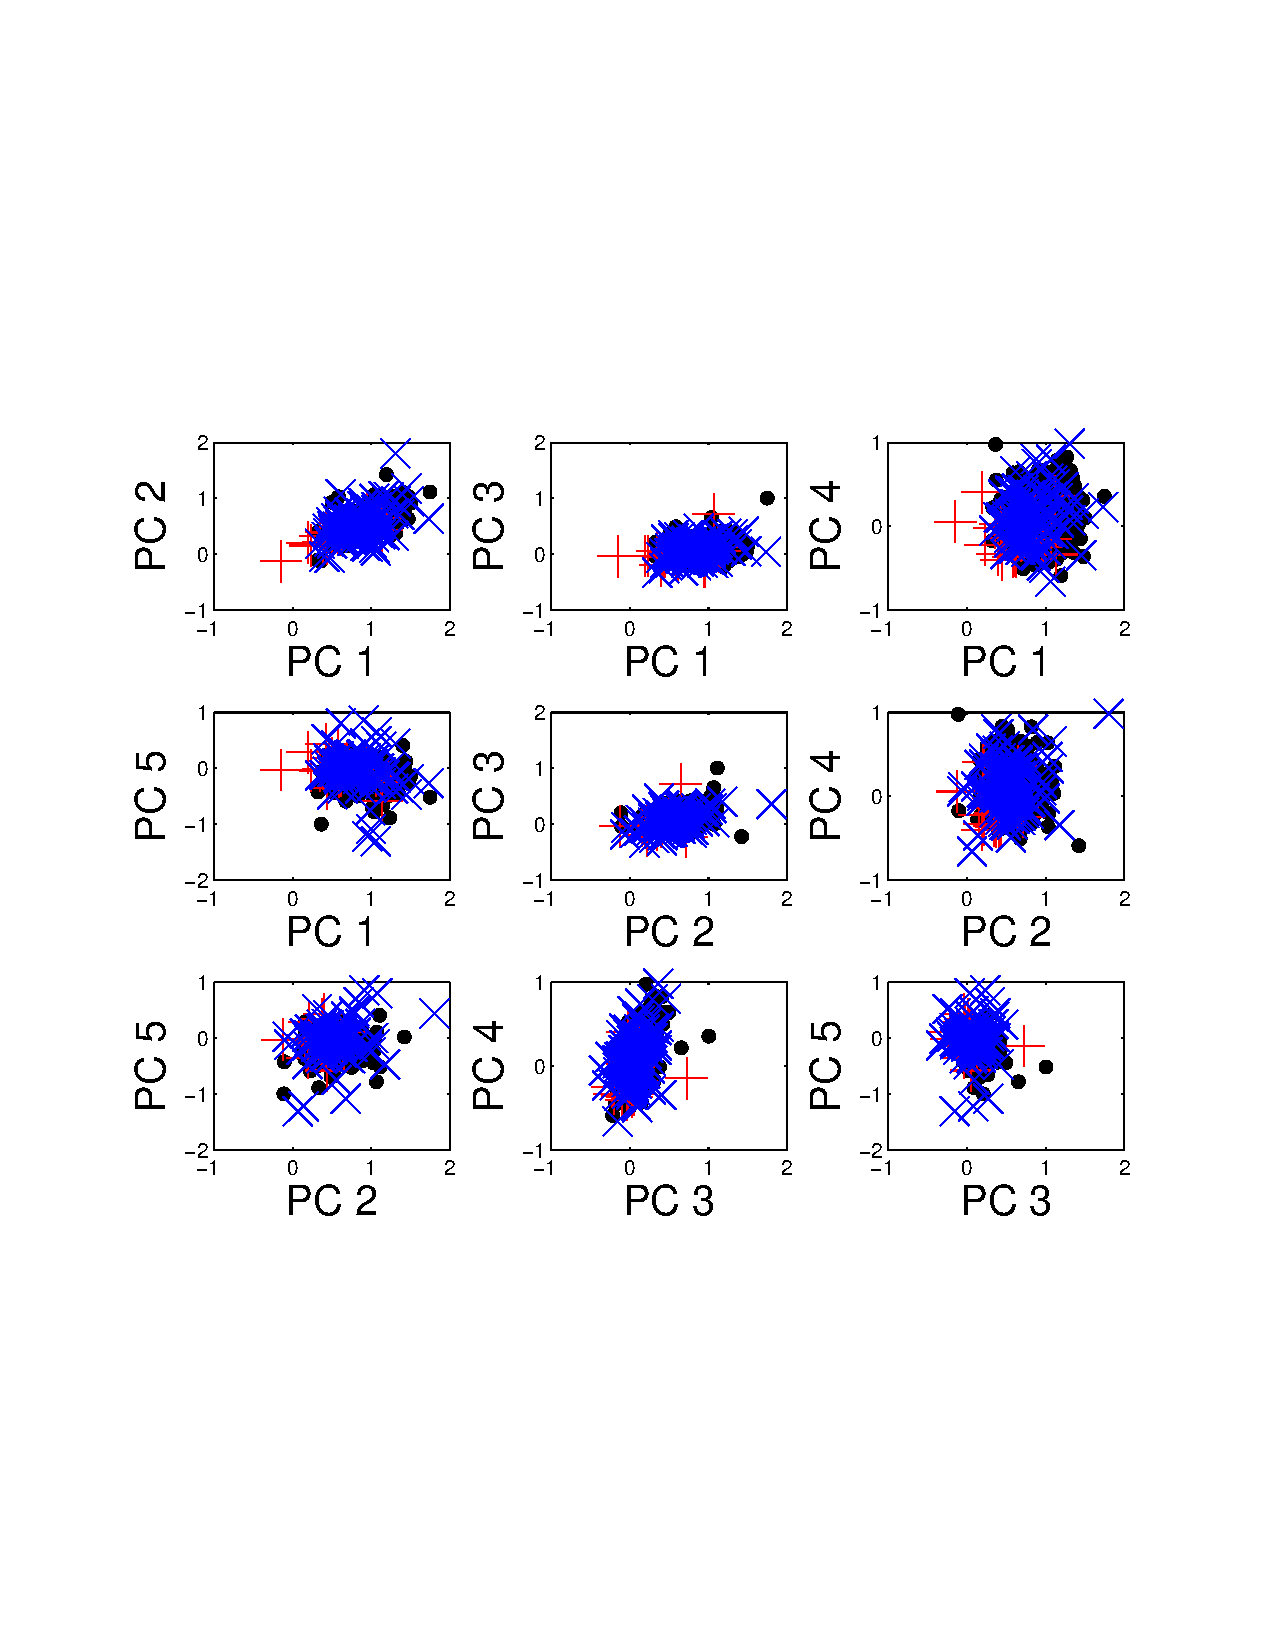
\includegraphics[height=3in]{../figs/new/pairs.pdf}
	\caption{(a) This shows the average number of true positives versus the average number of false positives in the intracellular cluster for 2 minute segments of the 4 minutes of the experiment.  \smug\ does better than    \jovo{let's make the symbols different for the different methods.  also, let's make the axes in terms of percentages, rather than raw numbers.} }
	\label{fig:pairs}
\end{figure}


\begin{figure}[htbp]
	\centering
		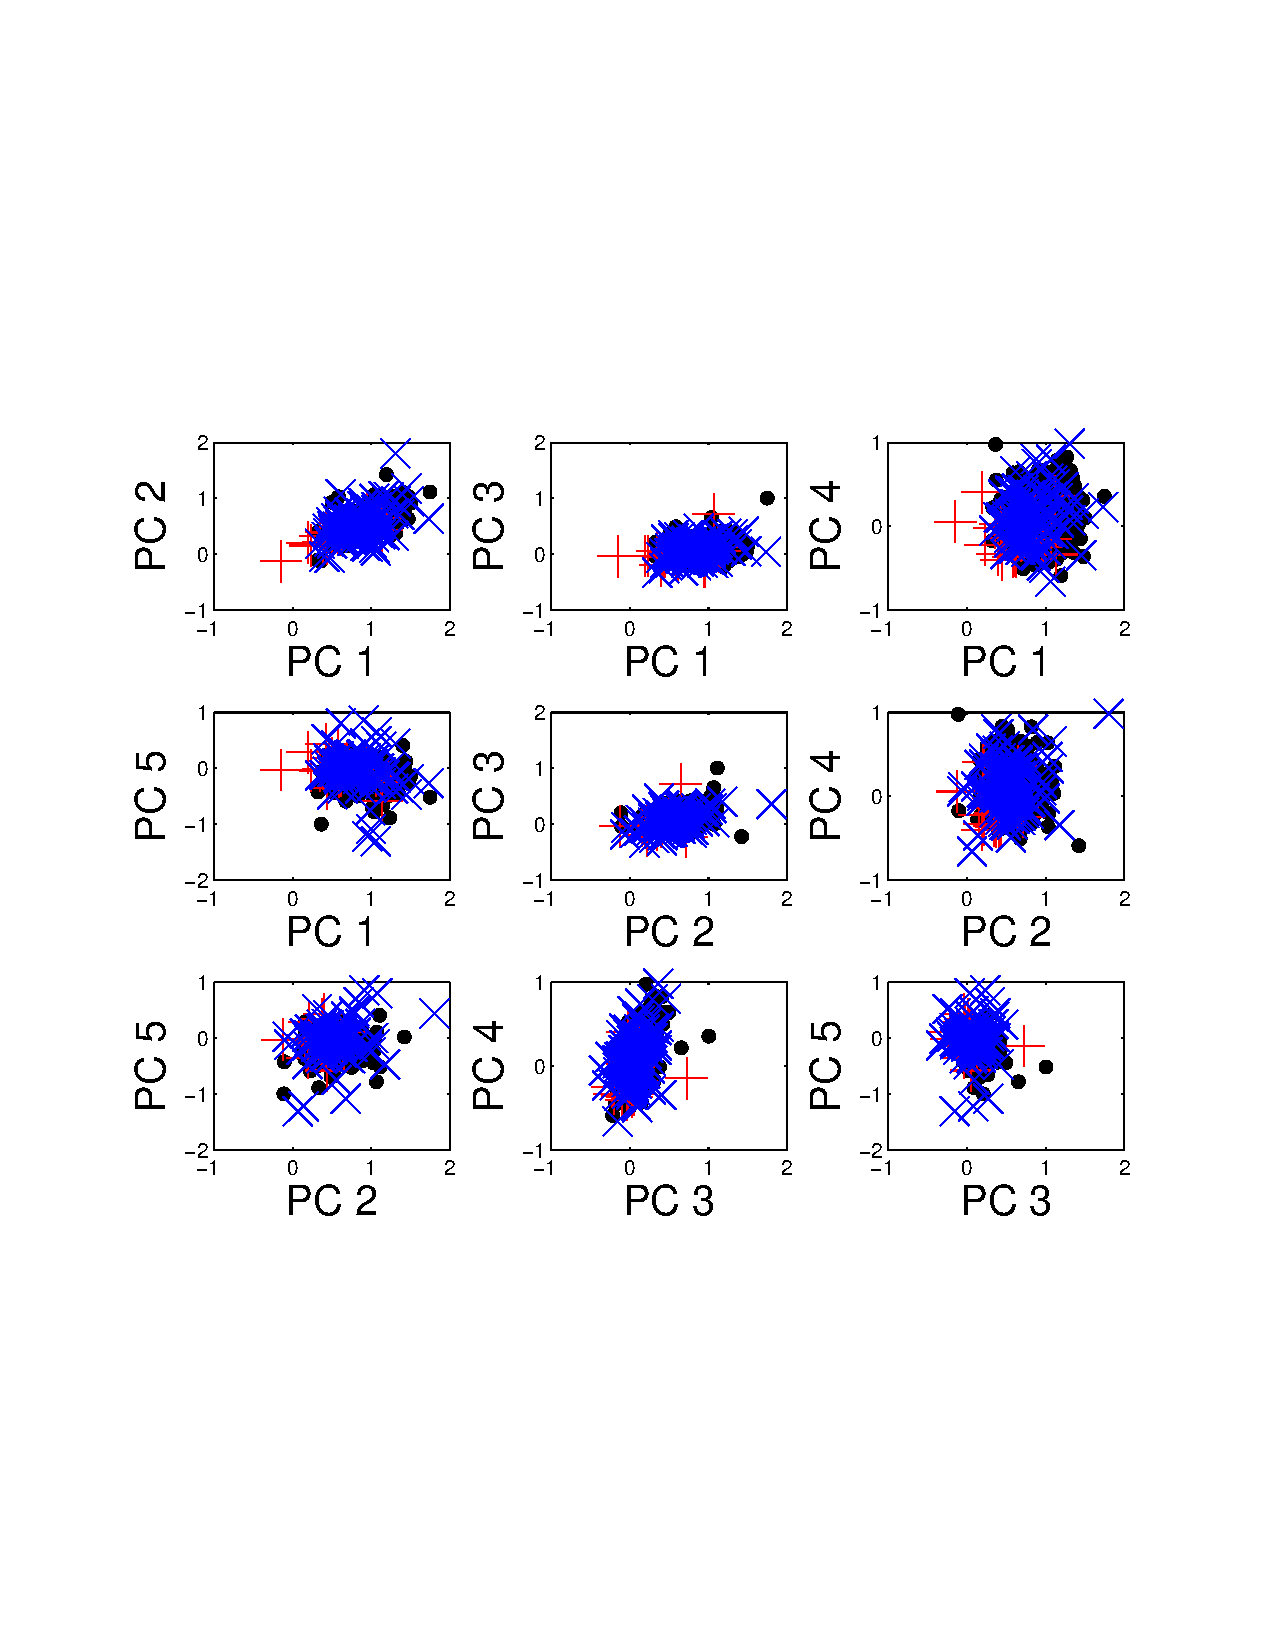
\includegraphics[height=3in]{../figs/new/pairs.pdf}
	\caption{caption}
	\label{fig:pairs}
\end{figure}
